\documentclass[UTF8,11pt,oneside]{ctexart}

\def\articletitle{因捍卫言论自由逃离俄罗斯后,电报创始人被法国逮捕}
\usepackage{CJKfntef}
\usepackage{float}

\usepackage{geometry}
\geometry{a4paper,left=2cm,right=2cm,top=2cm,bottom=1cm}

\usepackage{graphicx}

\usepackage{hyperref}
\hypersetup{colorlinks=true, linkcolor=red}

\linespread{1.6}

\usepackage{fancyhdr}
\usepackage{ifthen}
\pagestyle{fancy}
\fancyhf{}
\setlength{\headheight}{14pt}
\fancyhead[R]{\ifthenelse{\value{page}>1}{\thepage}{}}
\fancyhead[C]{\ifthenelse{\value{page}>1}{\articletitle}{}}
\renewcommand\headrulewidth{0pt}

\usepackage{tcolorbox}
\tcbuselibrary{skins}

\newcommand{\zd}[1]{\textbf{\textcolor[RGB]{123,12,0}{#1}}} % 重点

\newcommand{\yinyong}[1]{% 引用
    \begin{tcolorbox}[enhanced,
        frame hidden, interior hidden,
        before skip = 5mm, left skip=10mm,
        borderline west={5pt}{0pt}{gray!50}]
        #1
    \end{tcolorbox}
}

\newcommand{\xhx}[1]{%下划线(模拟微信中的划线功能,用于标注我个人认为的文章中精彩的地方)
    \CJKunderline*[thickness=1.5pt, format=\color[RGB]{84,216,140}]{#1}
}

\newcommand{\biaoti}[1]{% 标题
    \section*{#1}
}

\newcommand{\SetSectionType} {
    \ctexset{
        section={
            number = \chinese{section},
            aftername={、},
            format=\Large\bfseries,
        }
    }
}



\begin{document}

\begin{center}
    \LARGE{\articletitle\footnotemark}
\end{center}
\footnotetext{
    原文出自公众号“远方青木”的文章 《\href{https://mp.weixin.qq.com/s/zfU4x8jZSG9zU_ot1zfUDg}{\articletitle}》
}

帕维尔·杜罗夫,俄罗斯及独联体国家最大社交网站VKontakte(简称VK)的创始人,世界著名即时加密通讯软件Telegram(简称电报或纸飞机)的创始人。

杜罗夫出生在前苏联,拥有俄罗斯国籍,4岁时和家人移居到意大利,2006那年21岁的杜罗夫回到俄罗斯创办了VK,业界称这款软件为俄罗斯版脸书。

\zd{2011年,俄罗斯要求杜罗夫配合对反政府人士进行言论审查,杜罗夫的回应是公开在网上发布一张照片,对普京竖起了中指。}

\begin{figure}[H]
    \centering
    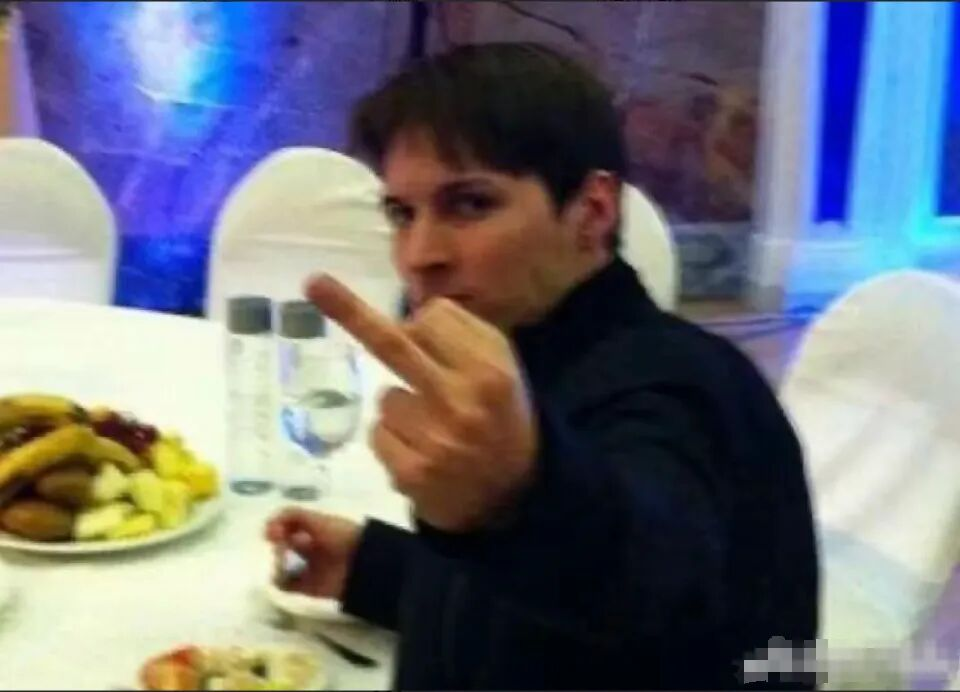
\includegraphics[width=12cm]{2024-08-28-001.jpg}
\end{figure}

随后乌克兰开始酝酿颜色革命,大量煽动者在VK上发布信息,导致了事态的急剧失控。

2013年,俄罗斯以严重危害国家安全为由,要求VK交出乌克兰颜色革命中的煽动者名单,杜罗夫的回应是直接出售股份,卖掉了VK公司。

\zd{杜罗夫坚决不从的原因是他认为必须捍卫言论自由,有煽动者利用VK平台搞破坏确实不对,但那也是煽动者的言论自由,你如果觉得这不对可以自由发表自己的言论辩回去,真理越辩越明,要求平台交出煽动者名单来对一些人强行闭嘴这是绝对不可能的事情。}

胳膊拧不过大腿,如果俄罗斯非要名单,那VK公司我就不要了,拿钱走人,因为触犯了杜罗夫的底线,也就是言论自由。

俄罗斯也没为难杜罗夫,对普京竖起中指那也是杜罗夫的言论自由,俄罗斯要的只是一个不被煽动者利用的VK平台,至于出售VK公司股份的钱,一分不少的给杜罗夫,要走也不拦着。

\zd{当年欧美媒体写了很多文章,盛赞杜罗夫是一位民主自由的斗士,因为受到了俄罗斯的迫害而被迫出走。}

2013年离开俄罗斯后,杜罗夫创办了Telegram实时通讯软件(电报),以绝对捍卫言论自由为主要卖点。

有多言论自由?

电报拒绝任何国家任何形式的言论审查,不对用户所有形式的交流进行任何形式的干涉,是真的不窃取和保留用户的数据,只要不被其他用户大量举报,你的任何东西都可以留存,你设置几天消除的信息,到期就真的烟消云散,世界上从未出现过电报用户信息被任何国家和组织查看过的事情。

这个社交软件自由到根本不打什么擦边球,里面的大量用户明着违法,什么黄色、赌博、毒品、血腥、电诈、黑帮交流乃至于恐怖主义等严重违法信息在里面铺天盖地。

\zd{杜罗夫认为,虽然他们的言论可能有问题,但这都是言论自由的一部分,电报平台以及任何国家都没资格审查。}

整个电报平台,实际上就是公开的暗网,里面藏污纳垢,是各路犯罪组织的乐园。

但因为电报不受任何国家言论审查的特点,成了西方组织颜色革命的利器,所有国家的颜色革命中都有电报平台的身影,其绝对捍卫言论自由的态度让颜色革命的组织者基本都选择在电报群里发号施令。

在乌克兰、中东、东亚的各种骚乱事件中,电报平台曾被西方盛赞为通往“自由世界”的钥匙。

其他国家的大家可能不熟悉,但在2019年,香港的黑暴份子就是在电报群里发布路障和燃烧弹的制作办法,报告警察实时位置、转发仇警图片及假新闻,每日聚集的时间和地点以及当日目标等信息,全部都在电报群里进行。

为规避各国监管,杜罗夫给自己弄了个阿联酋的国籍,并长期呆在那里。

以不到30个员工的数量,杜罗夫的电报平台支撑了接近10亿用户的使用,服务器的硬件支出成了唯一的成本,而电报平台也以2100亿人民币的估值入选了胡润全球独角兽榜。

2021年,法国决定授予帕维尔·杜罗夫 (Pavel Durov) 法国荣誉公民身份,以表彰他为言论自由做出的奋斗和贡献。

对于这一荣誉,杜罗夫欣然接受,并同时自动获得了法国国籍。

看起来,似乎对杜罗夫本人来说是好事。

但2023年10月,巴以冲突再次爆发,这次以色列不仅没有迅速扫荡掉哈马斯,还陷入了艰苦的持久战。

随着战争的持续,随着以色列对加沙平民的血腥屠杀,越来越多的反犹声音在欧美世界诞生,并在多个平台迅速蔓延。

不管是油管还是脸书还是X平台,都是受到欧美政府严格监管的,对相应的反犹声音都有限制。

但电报群不受任何国家监管,对言论自由绝对捍卫,于是这些反犹声音最后都汇聚到电报群里,然后在里面互相共振。

对于杜罗夫和电报平台,欧美政府一开始是打算好好谈的,能和平解决此事最好,毕竟言论自由可是一个金字招牌,还是挺值钱的,于是私下找到了杜罗夫进行沟通。

但没有想到杜罗夫这个人不是因为反俄而逃离俄罗斯,也不崇拜欧美,他是真的坚信言论自由,对美国抛出的橄榄枝不屑一顾,又臭又硬。

2024年4月,杜罗夫在接受采访时公开说:

\yinyong{Telegram引起了美国情报部门关注,后者曾向他了解该平台的情况,还试图秘密招募Telegram技术人员,美国政府可能想在Telegram安装一个“后门”,访问平台系统和数据库……}

对着全球说美国政府想在电报平台里装后门,肆意查阅电报用户的数据,话说到这份上那脸就彻底撕破了,美国政府也就没什么好和杜罗夫谈的了。

\xhx{在其他国家搞颜色革命时发挥重要作用,那杜罗夫当然是在捍卫言论自由,但在美国高校声援巴勒斯坦的抗议活动中也发挥重要作用,对各路反犹声音丝毫不加以监管和控制,这可就绝对不是什么言论自由了。}

后来一群“反以黑客”通过黑客技术,获取了大量有关以色列和犹太资本的黑料,高达数十G,以色列政府对此要求电报平台予以删除,且提供爆料人的信息,同时接受以色列政府的言论审查。

对此要求电报平台直接拒绝,此事成为了引爆矛盾的导火索。

8月24日晚,杜罗夫从阿塞拜疆乘坐私人飞机抵达法国巴黎勒布尔热机场时,被法国情报部门当场逮捕。

此事震惊了世界,因为杜罗夫长期以来被视为言论自由的代表,是欧美吹捧了十多年的自由斗士,在颠覆诸多反美国家的颜色革命里立下汗马功劳。

\zd{就算真要抓杜罗夫,那也不应该是欧美世界来抓,法国出面来抓杜罗夫真的是颠覆了全世界的三观。}

当然法国抓捕杜罗夫的罪名并不是言论自由,而是以恐怖主义、非法毒品交易、欺诈、洗钱和儿童色情等罪名来指控杜罗夫,最高将对杜罗夫判刑20年。

其指控逻辑是这样的,因为有恐怖份子在电报群里发布恐怖信息,而杜罗夫无法证明自己并非这些恐怖份子的组织者,也无法证明自己并非是这些恐怖信息的故意发布者,所以有理由怀疑杜罗夫涉嫌恐怖犯罪。

而里面是非法毒品交易和儿童色情犯罪信息等也是同样的逻辑,我现在怀疑这些信息就是你杜罗夫发布的,只是假借了电报平台一个虚拟用户的名义,所以你杜罗夫涉嫌犯罪,除非你能提供充足的证据来“证明”你自己并非这些犯罪信息的发布者。

法律逻辑也明确,意思也很明确,就是要电报平台的用户信息,且以后时刻接受欧美的言论审查。

不接受,那就关20年,接受了就可以和解,配合到位那罚点款接受点教训就可以回家了,这也是明牌。

至于为什么是法国来抓?

因为2021年的时候法国以杜罗夫为言论自由做出了巨大贡献为由授予了其法国荣誉荣民的身份,所以杜罗夫具有了法国国籍,所以2024年的时候法国可以直接抓捕法国公民杜罗夫,因为杜罗夫坚决捍卫言论自由。

真是天大的讽刺。

电报平台存在毒品和色情交易,以及大量恐怖主义信息,此事是确凿无疑的,但一直以来电报平台都是如此啊,做同样的事情,怎么以前就是捍卫言论自由的斗士,如今就是违法犯罪的嫌疑人?

\begin{figure}[H]
    \centering
    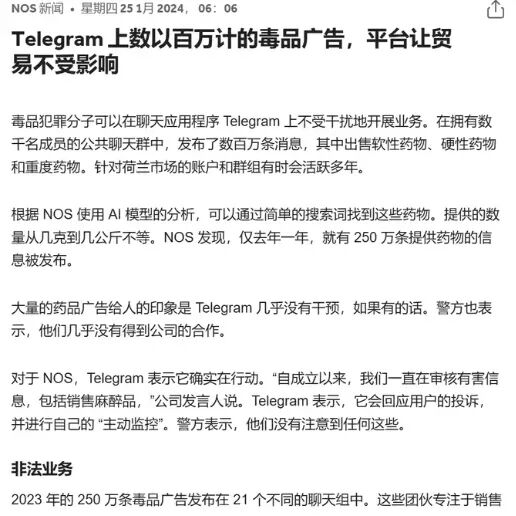
\includegraphics[width=10cm]{2024-08-28-002.jpg}
\end{figure}

杜罗夫被抓后,意大利副总理泰奥·萨尔维尼8月25日在Facebook上预测,下一个“被迫闭嘴”的人可能会是X平台所有者马斯克。

\begin{figure}[H]
    \centering
    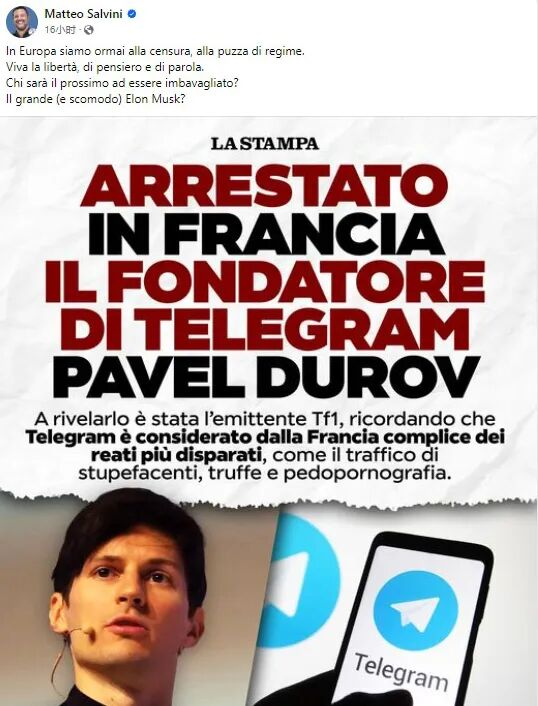
\includegraphics[width=10cm]{2024-08-28-003.jpg}
\end{figure}

而马斯克对此事的反应也异常强烈,他对此连续发言称:

\yinyong{
    “帕维尔·杜罗夫今晚被关进了法国监狱,对于那些拒绝在政府和情报机构的要求下审查真相的平台所有者来说,这是活生生的警告。黑暗正迅速降临到这个曾经自由的世界。”


    “拘捕杜罗夫是保护言论自由的美国宪法第一修正案的很有说服力的广告”。


    “这是2030年的欧洲,你因为给梗图点赞被判死刑。”
}

\zd{但也就这些支持了,对杜罗夫该抓还是抓,毕竟这是欧美世界的国家意志。}

\begin{figure}[H]
    \centering
    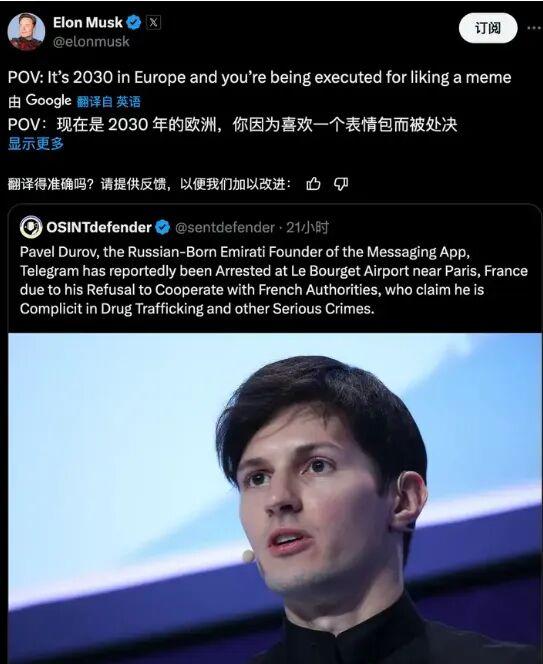
\includegraphics[width=11cm]{2024-08-28-004.jpg}
\end{figure}

\zd{唯一出面要保杜罗夫的,反而是以前被杜罗夫竖起中指的俄罗斯。}

8月25日凌晨,俄罗斯国家杜马副主席达万科夫呼吁俄罗斯外交部设法解救杜罗夫,他表示已经向俄罗斯外交部长拉夫罗夫发出了相应的请求。俄罗斯外交部表示,俄罗斯驻法国大使馆已经采取了必要措施,以了解帕维尔·杜罗夫的有关情况。

俄罗斯有权干涉杜罗夫,是因为杜罗夫具有俄罗斯国籍,但法国也有权拒绝,因为杜罗夫也有法国国籍,法国把一个犯罪的法国人关进监狱不需要得到俄罗斯的同意。

\xhx{以前都说具备多国国籍就成了世界公民,哪都能去,但现在看,具备多国国籍的后果就是哪国都能抓你,然后背后没有任何国家会真正为你撑腰。}

\zd{和平和乱世,是不一样的规则。}

在杜罗夫被抓后,俄罗斯前总统梅德韦杰夫在杜罗夫创建的电报Telegram上写道:

\yinyong{“很久以前,我问过杜罗夫,为什么他不愿意在严重犯罪的问题上与执法机构合作?他当时回答说,‘这是我的原则立场’。但我告诉他,‘这样会在任何国家都碰到严重的问题’。”

    “他认为自己最大的问题就是身处俄罗斯,于是他离开了,然后又获得了其他国家的国籍或居住许可。他想成为一个出色的‘世界公民’,即便没有祖国也能过着美好的生活。如拉丁谚语云:Ubi bene ibi patria!哪里过得好,哪里就是祖国。”


    “但他失算了。对于所有我们现在共同面对的敌人来说,他就是俄罗斯人,因此是不可预测且危险的,他身上流着不一样的血。”


    “他不是马斯克,也不是扎克伯格(顺便说一句,他们还积极与美国联邦调查局合作)。”


    “\xhx{杜罗夫最终应当明白,祖国和时代一样,都是无法选择的……}”
}

俄罗斯力挺杜罗夫,固然有法国抓捕杜罗夫后这么做可以有效打击欧美世界言论自由的金字招牌的政治考虑。

但做事论迹不论心,单论做出来的事情,那就是杜罗夫对普京竖中指,放任反俄信息在自己创建平台上肆意传播,帮欧美世界把舆论战前线推进到了俄罗斯心腹地带,对俄罗斯的一切请求拒不配合,这些年来为欧美世界在各国搞颜色革命立下了汗马功劳。

\zd{最后是欧美国家出面抓捕了杜罗夫并威胁要判刑20年,而唯一出面要保杜罗夫的国家反而是俄罗斯。}

别管做出这些决定的时候都是出于什么因素考量的,但这些就是最终欧美国家和俄罗斯做出来的客观事实。

\zd{到底谁才是真正言论自由的国家?}

\zd{京子心善,这已经快不是一个梗了,最近几年在欧美世界的衬托下已经越来越成为了现实。}

\zd{杜罗夫作为一个俄罗斯人,可以反俄,但不能反美,更不能反犹。}

如果杜罗夫反俄,那俄罗斯还会对杜罗夫手下留情,但如果杜罗夫敢反美甚至反犹,那欧美世界绝对不会手下留情。

拒绝给俄罗斯提供用户信息,全网公开对普京树中指,好多年都没事,要走不拦,带钱走也行,但仅仅是不给美国及以色列提供ID,几个月就进去了。

赵长鹏,出生在中国,后加入加拿大国籍,并设法取得了阿联酋公民身份,创立加密货币交易平台币安,被抓。

杜罗夫,出生在俄罗斯,后加入法国国籍,并设法取得了阿联酋公民身份,创立加密即时通讯平台电报,被抓。

这些人以为拥有阿联酋公民身份就可以规避各国监管,但只要触犯了美国利益,就会直接被抓。

\yinyong{
    “他总仍旧是偷。这一回,是自己发昏,竟偷到丁举人家里去了。他家的东西,偷得的么?”

    “后来怎么样?”

    “怎么样?抓到大狱里,先画押认罪,后来是打,打了大半夜,再打折了腿。”

    “后来呢?”

    “后来打折了腿了。”

    “打折了怎样呢?”

    “怎样?……谁晓得?也许是死了。”

    掌柜也不再问,仍然慢慢的算他的账。
}

现在的欧美媒体已经都在报道电报平台的各种犯罪事迹,说的确实都是事实,因为这种犯罪事迹在电报平台上一抓一大把。

事都是这些事,但你想象一下,如果是俄罗斯抓捕了杜罗夫,你猜欧美的媒体会怎么报道?

\zd{当侵犯别人利益的时候,欧美世界高举言论自由的大旗。}

\zd{当自己的利益被侵犯时,欧美世界直接下场抓人,这不仅仅是针对电报平台。}

在法国抓捕电报创始人杜罗夫的同时,英国一位记者仅仅因为批评以色列对加沙实行了种族灭绝,就说了几句话,下飞机就直接被英国逮捕了,面临刑事指控。

\begin{figure}[H]
    \centering
    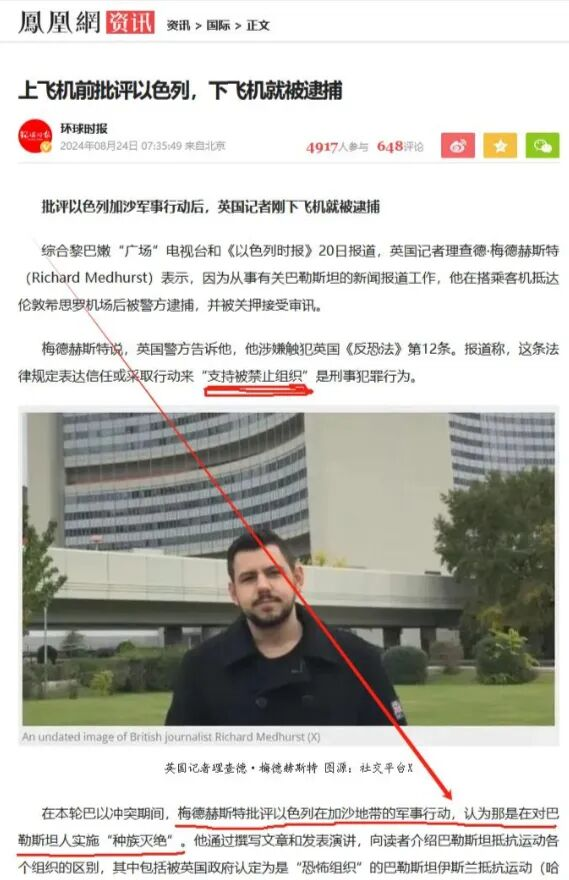
\includegraphics[width=9cm]{2024-08-28-005.jpg}
\end{figure}

国名一换,那直接就是评论过万啊,怎么这种严重侵犯言论自由的事情别的国家都不做,就法国和英国能做,还敢做?

\begin{figure}[H]
    \centering
    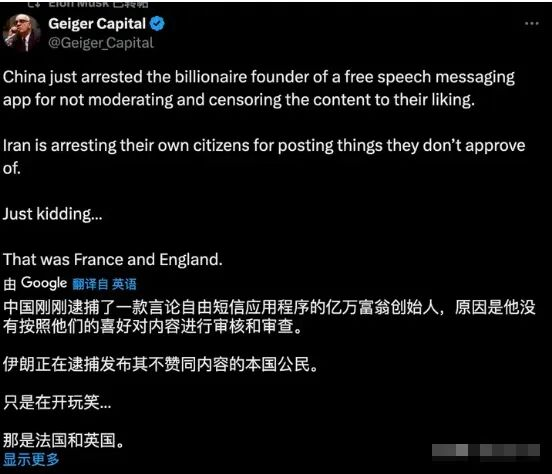
\includegraphics[width=10cm]{2024-08-28-006.jpg}
\end{figure}

利益,是评价政治行为的永存标准,这是大学课本上国际政治的六原则之一。

\begin{figure}[H]
    \centering
    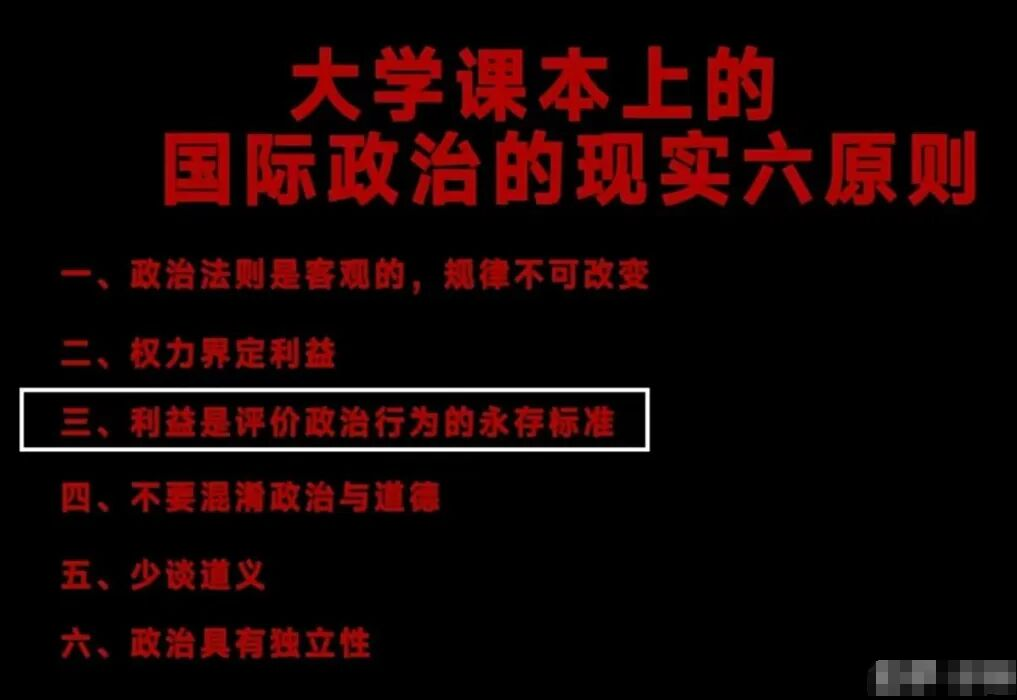
\includegraphics[width=10cm]{2024-08-28-007.jpg}
\end{figure}

所以法国在2021年以为捍卫言论自由做出巨大贡献授予杜罗夫荣誉公民的身份,并在2024年以捍卫言论自由为由抓捕法国公民杜罗夫,看起来前后矛盾,但根据国际政治六原则,这其实一点都不矛盾,都是为了利益,至于什么言论自由那只是个幌子和由头。

\zd{但在利益决定政治行为的政治原则之外,也有温情的成分,那就是血缘、种族和母国,这些是可以在一定范围内超越利益之上的。}

\zd{梅德韦杰夫有句话我觉得说的很好,那就是杜罗夫最终应当明白,祖国和时代一样,都是无法选择的。}

\zd{此番从法国的大牢里出来后,无论最终是什么形式出来的,有没有对欧美屈服,我相信杜罗夫都应该能理解这句话了。}

\end{document}

